\section{Introduction}

\begin{frame}
	\frametitle{Discretization of Continuous-time systems}
	\begin{block}{Use of discretization}
		Many systems in the real world are continous systems: chemical reactions, rocket trajectories, power plants, ice cap melting... Computers, however, are mainly digital. If we want to simulate the continuous system with a digital device, we need a method to convert the continuous model into a discrete one.  This conversion is called "discretization" or "sampling". Discretization also comes in handy when a continuous filter with usefull properties has been designed and a discrete filter with the same properties is required.
	\end{block}
\end{frame}

\begin{frame}
	\frametitle{Discretization}
	\begin{block}{Problem statement}
		While converting, some information of the continuous model will be lost due to the different nature of the systems. It is important that the loss of information is minimized. Each discretization method has its own qualities and they will all lead to different discrete representations of the same continuous system.
	\end{block}
	
	\begin{block}{Discretization methods discussed in this lecture}
		\begin{itemize}
			\item Numerical Integration
			\item Zero-pole equivalent
			\item Hold equivalents
		\end{itemize}
	\end{block}
\end{frame}

\section{Main Approaches}
\subsection{Numerical Integration}

\begin{frame}
	\frametitle{Numerical Integration}
	\begin{block}{General approach}
		The system transfer function H(s) is first represented by a differential equation. Next a difference equation, whose solution is an approximation of this differential equation, is derived: 
		\begin{center}
			$H(s) = \frac{a}{s + a}$
			is equivalent to the differential equation
			$\frac{\mathrm d}{\mathrm d t} \big( u(t) \big) + a*u(t) = a*e(t)$
			
			solving this equation results in the following integral
			$u(t) = \int_0^t \big(-a*u(\tau) + a*e(\tau) \big)\mathrm{d}\tau$
			
			$u(k*T) = u(k*T - T)+ $ \begin{cases}
				\text{area of  $-a*u(t) + a*e(t)$}\\
				\text{over $k*T - T \leq \tau < k*T$}
			\end{cases}
			$(8.1)$
		\end{center}
		Where T is the sampling time. The transfer function above will be used for all the numerical integration methods.
	\end{block}
\end{frame}

\begin{frame}
	\frametitle{Forward rectangular rule (=Forward Euler)}

	\begin{block}{General approach}
		The area is approximated by the rectangle looking \textbf{forward} from $(k*T - T)$ toward $k*T$ with an amplitude equal to the value of the function at $(k*T - T)$. A smaller step-size T leads to a more accurate approximation, as shown in the figures.
	\end{block}

\begin{columns}
	\begin{column}{0.5\textwidth}
		\begin{figure}
			\centering
			\includegraphics[width=0.6\linewidth]{Forward1}
		\end{figure}
	\end{column}
	
	\begin{column}{0.5\textwidth}
		\begin{figure}
			\centering
			\includegraphics[width=0.6\linewidth]{Forward2}
		\end{figure}
	\end{column}
\end{columns}
\end{frame}

\begin{frame}
	\frametitle{Forward rectangular rule}
	\begin{block}{Mathematical approach}
		The general approach (formula (8.1)) applied on the forward rectangle rule, results in an equation $u_1$:
		\begin{align*}
		u_1(k*T)& =u_1(k*T - T) + T*\big(-a*u_1(k*T - T)\\
		& + a*e(k*T - T) \big)\\
		& =(1 - a*T)*u_1(k*T - T) + a*T*e(k*T - T)
		\end{align*}
	\end{block}
\end{frame}

\begin{frame}
	\frametitle{Forward rectangular rule}
	\begin{block}{Mathematical approach}
		In this case, the transfer function is:
		\begin{center}
		$H_F(z) = \frac{a}{(z-1)/T+a}$
		\end{center}
		Which can also be derived using the following substitution in the given transfer function:
		\begin{center}
			$s \gets \frac{z-1}{T}$ (8.2)
		\end{center}
		This is extremely usefull while making exercises.
	\end{block}
\end{frame}	

\begin{frame}
	\frametitle{Backward rectangular rule (=Backward Euler)}
\begin{block}{General approach}
	The area is approximated by the rectangle looking \textbf{backward} from $k*T$ toward $(k*T - T)$ with an amplitude equal to the value of the function at $k*T$. 
\end{block}	

\begin{columns}
	\begin{column}{0.5\textwidth}
		\begin{figure}
			\centering
			\includegraphics[width=0.6\linewidth]{Backward1}
		\end{figure}
	\end{column}
		
	\begin{column}{0.5\textwidth}
		\begin{figure}
			\centering
			\includegraphics[width=0.6\linewidth]{Backward2}
		\end{figure}
	\end{column}
		
\end{columns}
\end{frame}

\begin{frame}
	\frametitle{Backward rectangular rule}	
	\begin{block}{Mathematical approach}
		The general approach (formula (8.1)) applied on the forward rectangle rule, results in an equation $u_2$:
		\begin{align*}
		u_2(k*T)& =u_2(k*T - T) + T*\big(-a*u_2(k*T) + a*e(k*T) \big)\\
		& =\frac{u_2(k*T - T)}{1 + a*T} + \frac{a*T}{1 + a*T}*e(k*T)
		\end{align*}
	\end{block}
\end{frame}

\begin{frame}
	\frametitle{Backward rectangular rule}
	\begin{block}{Mathematical approach}
		In this case, the transfer function is:
		\begin{center}
			$H_B(z) = \frac{a}{(z-1)/T*z+a}$
		\end{center}
		Which can also be derived using the following substitution in the given transfer function:
		\begin{center}
			$s \gets \frac{z-1}{T*z}$ (8.3)
		\end{center}
		Again this is extremely usefull while making exercises.
	\end{block}
\end{frame}

\begin{frame}
	\frametitle{Trapezoidal rule (= bilinear or Tusting rule)}
	
\begin{columns}
	\begin{column}{0.5\textwidth}
		\begin{block}{General approach}
			This method makes use of the area of the \textbf{trapezoid} formed by the average of the selected rectangles used in the forward en backward rectangle rule.Thus the amplitude equal to the value of the function at $(k*T - T)$ and the amplitude equal to the value of the function at $(k*T)*$ are connected by a line as shown in the illustration.
		\end{block}	
	\end{column}

	\begin{column}{0.5\textwidth}
		\begin{figure}
			\centering
			\includegraphics[width=1\linewidth]{Trapezium}
		\end{figure}
	\end{column}	
	
\end{columns}
\end{frame}

\begin{frame}
	\frametitle{Trapezoidal rule}
	\begin{block}{Mathematical approach}
		The general approach (formula (8.1)) applied on the forward rectangle rule, results in an equation $u_3$:
		\begin{align*}
		u_3(k*T)& =u_3(k*T - T) + T/2*\big(-a*u_3(k*T - T)\\
		& + a*e(k*T - T) - a*u_3(k*T) + a*e(k*T)\big)\\
		& =\frac{1-(a*T/2)}{1 + (a*T/2)}*u_3(k*T - T)\\
		& +\frac{a*T/2}{1 + (a*T/2)} * \big(e_3(k*T - T) + e_3(k*T)\big)
		\end{align*}
	\end{block}
\end{frame}

\begin{frame}
	\frametitle{Trapezoidal rule}
	\begin{block}{Mathematical approach}
		In this case, the transfer function is:
		\begin{center}
			$H_T(z) = \frac{a}{\frac{2}{T}*\frac{z-1}{z+1} * a }$
		\end{center}
		Which can also be derived using the following substitution in the given transfer function:
		\begin{center}
			$s \gets \frac{2}{T} * \frac{z-1}{z+1}$ (8.4)
		\end{center}
		This is extremely usefull while making exercises.
	\end{block}
\end{frame}

\begin{frame}
	\frametitle{Trapezoidal rule}
	\begin{example}
		Given:
		\begin{center}
			$H(s) = \frac{s + 1}{0.1*s + 1}$
		\end{center}
		We now apply substitution (8.4):
		\begin{center}
			$H(z) = \frac{(2 + T)*(T - 2)*z^{-1}}{(0.2 + T) + (T - 0.2)*z^{-1}}$
		\end{center}
		Using T=0.25s, this results in:
		\begin{center}
			$H(z) = \frac{5*(z - 0.7778)}{z + 0.1111}$
		\end{center}
	\end{example}
\end{frame}

\begin{frame}
	\frametitle{Stability of the numerical integration methods}
	\begin{block}{Stability}
		As already mentioned, a continuous system is stable when its poles have a negative real part in the s-plane and a discrete system is stable when its poles lie within the unit circle of the z-plane.Subsequently the $(s=j\omega)$-axis is the boundary between poles of stable and unstable continuous systems. Each of the discretization methods can be considered as a map from the s-plane to the z-plane. It is interesting to know how the $j\omega$-axis is mapped by every rule and where the stable part of the s-plane appears in the z-plane. This can be realized by solving formulas (8.2-8.3) to z and replacing s by $j\omega$. 
	\end{block}
\end{frame}

\begin{frame}
	\begin{block}{Graphical representation}
	\begin{figure}
		\centering
		\includegraphics[width=1\linewidth]{Stabiliteit}
	\end{figure}
	\end{block}
\end{frame}


\begin{frame}
	\frametitle{Bilinear rule with prewarping}
	\begin{alertblock}{Disortion}
		The bilinear rule maps the stable region of the s-plane into the stable region of the z-plane and the entire $j\omega$-axis is compressed into the $2\Pi$-length of the unit circle, causing a great deal of distortion. 
	\end{alertblock}
	
	\begin{block}{Trapezoid rule with prewarping}
		By extending the trapezoidal rule one step we can correct the distortion of the real frequencies mapped by the rule. This results in following substitution formula:
		\begin{center}
			$s \gets \frac{\omega_0}{tan\big(\frac{\omega_0 * T}{2}\big)} * \frac{z-1}{z+1}$ (8.4)
		\end{center}
	\end{block}
\end{frame}

\subsection{Zero-pole equivalent}

\begin{frame}
	\frametitle{Zero-pole equivalent}
	\begin{block}{General approach}
		The map $z = e^{sT}$ is applied to the poles as well as to the zeros of the continuous system. The following rules must be followed:
		\begin{enumerate}
			\item if $s=-a$ is a pole of H(s), then $z=e^{-a*T}$
			\item all finite zeros $s=-b$ are mapped by $z = e^{-b*T}$
			\item zeros at $\infty$ are mapped to $z = -1$
			\item the gain of the digital filter must match the gain of H(s) at the band center or a similar critical point.
		\end{enumerate}
	\end{block}
\end{frame}

\begin{frame}
	\frametitle{Zero-pole equivalent}
	\begin{example}
		Given:
		\begin{center}
			$H(s) = \frac{s + 1}{0.1*s + 1}$
		\end{center}
		Pole at $s=-10$ and zero at $s=-1$.
		
		New discrete transfer function with equivalent poles and zeros:
		\begin{center}
			$H(z) = K * \frac{z - e^{-1*T}}{z - e^{-10*T}}$
		\end{center}
		K is chosen so that $\mid H(z)\mid _{z=1} = \mid H(s) \mid _{s=0} \to K=4.150$

		Using $T=0.25$, this results in:
		\begin{center}
			$H(z) = 4.150 * \frac{z-0.7788}{z-0.0821}$
		\end{center}
	\end{example}
\end{frame}


\subsection{Hold equivalent}
\begin{frame}
	\frametitle{Hold equivalent}
	\begin{block}{General approach}
		This method uses a discrete system consisting of 3 subsystems, each with its own purpose. 
		\begin{enumerate}
			\item Hold: approximating $e_h(t)$ from the samples $e[k]$
			\item H(s): putting the $e_h(t)$ through the given transfer function H(s) of the continuous system, resulting in u(t)
			\item Sampler: sampling u(t) 
		\end{enumerate}
		\vspace{-1em}
		\begin{figure}
			\centering
			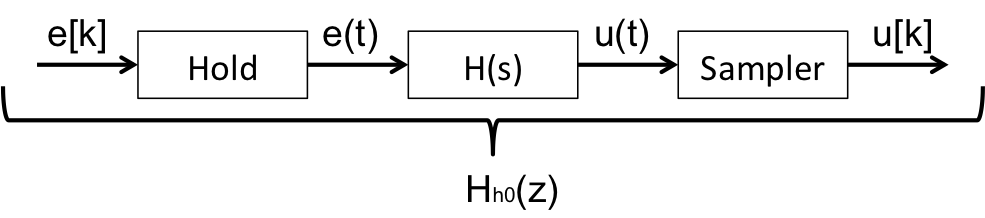
\includegraphics[width=0.8\linewidth]{hold_equivalent}
		\end{figure}
		\vspace{-1em}
		There are many techniques for holding a sequence of samples.
	\end{block}
\end{frame}

\begin{frame}
	\frametitle{Zero-order hold equivalent (ZOH)}
\begin{columns}
	\begin{column}{0.5\textwidth}
	\begin{block}{Practical rule}
		The zero-order hold equivalent transfer function $H_{zoh}(z)$ can be found by computing the following:
		\begin{center}
			$H_{zoh}(z) = (1 - z^{-1}) * \mathcal{Z}\{\frac{H(s)}{s}\}$
		\end{center}
	\end{block}
	\end{column}
	
	\begin{column}{0.5\textwidth}
		\begin{figure}
			\centering
			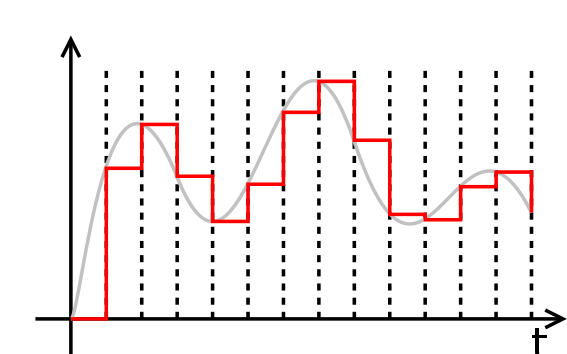
\includegraphics[width=1\linewidth]{zero-order}
		\end{figure}
	\end{column}
\end{columns}
\end{frame}

\begin{frame}
	\frametitle{Zero-order hold equivalent}
	\begin{example}
		\begin{center}
			$H(s) = \frac{0.1}{s + 0.1}$
		\end{center}
		Step 1: multiply by 1/s and perform partial fraction expansion
		\begin{center}
			$\frac{H(s)}{s} = \frac{0.1}{s * (s + 0.1)} = \frac{1}{s} - \frac{1}{s + 0.1}$
		\end{center}
		Step 2: perform z-transformation
		\begin{center}
			$\mathcal{Z} \{\frac{H(s)}{s}\} = \frac{1}{1 - z^{-1}} - \frac{1}{1 - e^{-0.1T} * z^{-1}}$
		\end{center}
		Step3: simplify and multiply by $(1-z^{1})$
		\begin{center}
			$H_{ho}(z) = \frac{1 - e^{-0.1T}}{z - e^{0.1T}}$
		\end{center}
	\end{example}
\end{frame}

\begin{frame}
	\frametitle{Non-causal first-order (= Triangle-hold equivalent (TRI))}
\begin{columns}
	\begin{column}{0.5\textwidth}
	\begin{block}{Practical rule}
		The non-causal first-order hold equivalent transfer function $H_{tri}(z)$ can be found by computing the following:
		\begin{center}
			$H_{tri}(z) = \frac{(z-1)^{2}}{T*z} * \mathcal{Z}\{\frac{H(s)}{s^{2}}\}$
		\end{center}
	\end{block}
	
	\begin{alertblock}{Non-causal vs causal}
		A causal first-order hold equivalent introduces a time-delay resulting in a less accurate approximation.
	\end{alertblock}
	\end{column}
	
	\begin{column}{0.5\textwidth}
		\begin{figure}
			\centering
			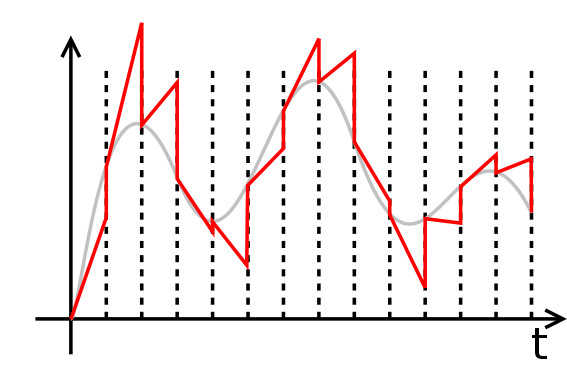
\includegraphics[width=1\linewidth]{first-order}
		\end{figure}
	\end{column}
\end{columns}
\end{frame}

\begin{frame}
	\frametitle{Triangle-hold equivalent}
	\begin{example}
		\begin{center}
			$H(s) = \frac{1}{s^{2}}$
		\end{center}
		Step 1: multiply by $1/s^{2}$ and perform partial fraction expansion
		\begin{center}
			$H(s) = \frac{1}{s^{4}}$
		\end{center}
		Step 2: perform z-transformation
		\begin{center}
			$\mathcal{Z}\{\frac{H(s)}{s^{2}}\} = \frac{T^{3}}{6} * \frac{(z^{2} + 4*z +1) * z}{(z-1)^{4}}$
		\end{center}
		Step 3: simplify and multiply by $\frac{(z-1)^{2}}{T*z}$
		\begin{center}
			$H_{tri}(z) = \frac{T^{2}}{6} * \frac{z^{2} + 4*z + 1}{(z-1)^{2}}$
		\end{center}
	\end{example}
\end{frame}

\begin{frame}
	\frametitle{Effect of zero- and first-order hold equivalents}
	\begin{block}{Effects on the spectrum}
		Some information will be permanentely lost.
		\vspace{-0.7em}
		\begin{figure}
			\centering
			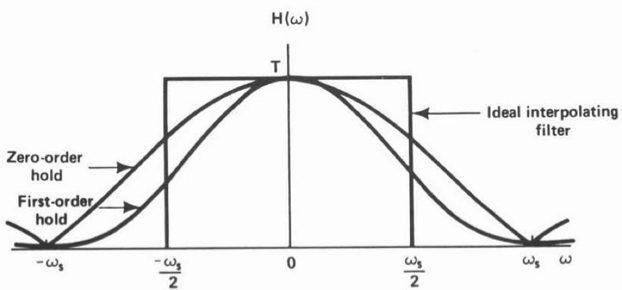
\includegraphics[width=1\linewidth]{effect_zoh_foh}
		\end{figure}
	\end{block}
\end{frame}

\section{Sampling Time}

\begin{frame}
	\frametitle{Sampling time T based on the frequency response}
	\begin{block}{Nyquist-Shannon sampling theorem}
		If a function $x(t)$ contains no frequencies higher than B hertz, it is completely determined by giving its ordinates at a series of points spaced $1/(2B)$ seconds apart. A sufficient sample-rate is therefore \textbf{2B samples/second}. This is called the \textbf{"Nyquist sampling rate"}. Equivalently, for a given sample rate $f_s$, perfect reconstruction is guaranteed possible for a bandlimit $B ≤ f_s/2$. 
	\end{block}
	\begin{block}{Practical rule}
		A higher sampling rate creates a margin of error, a good rule of thumb is \textbf{2,2B samples/second}.
	\end{block}
\end{frame}

\begin{frame}
	\frametitle{Sampling time T based on the time response}
	\begin{block}{Impuls response}
		If the time response is given, you need to calculate
	\end{block}
\end{frame}

\section{Discretization and Matlab}

\begin{frame}
	\frametitle{Matlab}
	\begin{block}{Matlab Command}
		Control System Toolbox™ offers extensive support for discretization and resampling of linear systems:
	\begin{itemize}
		\item "c2d(system,sampling time,method)" used for discretization
		\item "d2c(system,sampling time,method)" used for reconstruction
		\item "d2d(system,sampling time,method)" used for resampling
	\end{itemize}
	\end{block}
	
	\begin{block}{Available methods}
		\begin{itemize}
			\item zero-order hold equivalent: "zoh"
			\item first-order hold equivalent: "foh"
			\item bilinear: "tustin"
			\item zero-pole matching period: "matched"
		\end{itemize}
	\end{block}
\end{frame}

\begin{frame}
	\frametitle{Zero-order hold equivalent}
\begin{columns}
	\begin{column}{0.6\textwidth}
	\begin{example}
		Given:\\
		$H(s) = e^{-s} * \frac{s-2}{s^{2} + 3*s + 20} $\\
		sampling frequency = 10Hz\\
		\vspace{1em}
		Commands in Matlab:
		
		H = tf([1 -2],[1 3 20],'inputdelay',1); \\
		Ts = 0.1; \\
		Hd = c2d(H,Ts,zoh)\\
		\vspace{1em}
		Result:
		$Hd(z) = z^{-10} * \frac{(0.07462*z - 0.09162)}{z^{2} - 1,571*z + 0.7408}$
	\end{example}
	\end{column}
	
	\begin{column}{0.4\textwidth}
		\begin{figure}
			\centering
			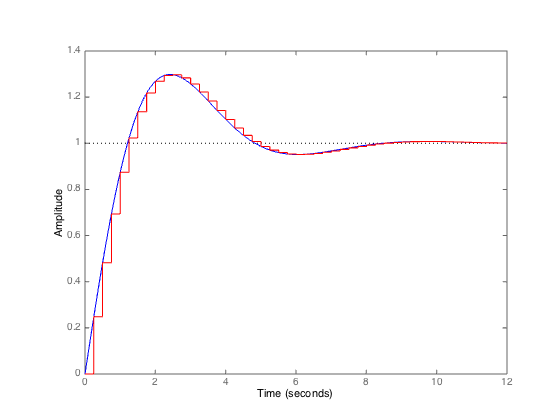
\includegraphics[width=1\linewidth]{vb1}
		\end{figure}
	\end{column}
\end{columns}
\end{frame}

\begin{frame}
	\frametitle{First-order hold equivalent}
\begin{columns}
	\begin{column}{0.6\textwidth}
	\begin{example}
	Given:\\
	$H(s) = e^{-0.3s} * \frac{s-1}{s^{2} + 4*s + 5} $\\
	sampling frequency = 10Hz\\
	\vspace{1em}
	Commands in Matlab:
	
	H = tf([1 -1],[1 4 5],'InputDelay', 0.3);\\
	Hd = c2d(H,0.1,'foh');\\
	Hd = c2d(H,Ts,zoh)\\
	\vspace{1em}
	Result:
	\end{example}
	\end{column}
	
	\begin{column}{0.4\textwidth}
		\begin{figure}
			\centering
			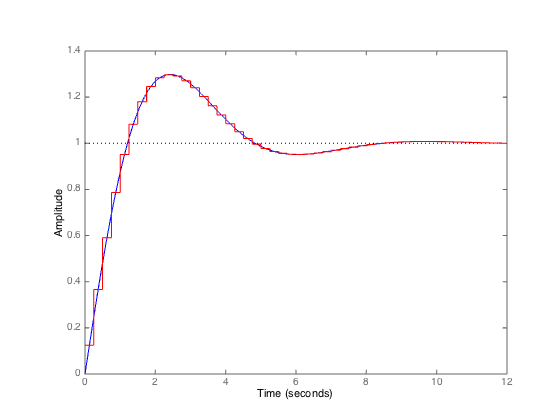
\includegraphics[width=1\linewidth]{vb2}
		\end{figure}
	\end{column}
\end{columns}
\end{frame}